\documentclass{article}

\usepackage{graphicx}
\usepackage{fancyhdr}
\usepackage{float}
\usepackage{pdfpages}
\usepackage[sorting=none]{biblatex}
\usepackage{listings}
\usepackage[hidelinks]{hyperref}
\usepackage{subfigure}
\usepackage{shapepar}
\usepackage{amsmath,amssymb}
\usepackage{pgfplots}
\pgfplotsset{compat=1.18}
\usepackage{xcolor}
\usepackage{booktabs}
\usepackage{caption}
\usepackage{setspace}
\usepackage[margin=2.5cm]{geometry}

\hypersetup{
	colorlinks=true,
	linkcolor=teal,
	filecolor=magenta,
	urlcolor=teal,
	citecolor=teal
}


\captionsetup{
	font=small,
	labelfont=bf,
	skip=6pt
}


\definecolor{codegreen}{rgb}{0,0.6,0}
\definecolor{codegray}{rgb}{0.5,0.5,0.5}
\definecolor{codepurple}{rgb}{0.58,0,0.82}
\definecolor{backcolour}{rgb}{0.96,0.96,0.94}
\definecolor{codeblue}{rgb}{0.13,0.29,0.53}

\lstdefinestyle{mystyle}{
	backgroundcolor=\color{backcolour},
	commentstyle=\color{codegreen}\itshape,
	keywordstyle=\color{codeblue}\bfseries,
	numberstyle=\tiny\color{codegray},
	stringstyle=\color{codepurple},
	basicstyle=\ttfamily\footnotesize,
	breakatwhitespace=false,
	breaklines=true,
	captionpos=b,
	keepspaces=true,
	numbers=left,
	numbersep=8pt,
	showspaces=false,
	showstringspaces=false,
	showtabs=false,
	tabsize=2,
	frame=single,
	rulecolor=\color{codegray},
	xleftmargin=12pt,
	framexleftmargin=12pt
}

\lstset{style=mystyle}
\renewcommand{\lstlistingname}{Code}


\usepackage{xepersian}
\setlength\headheight{28pt}
\settextfont[Path={./font/}, Scale=1.3]{IRLotus}
\setlatintextfont[Scale=1]{Times New Roman}
\setdigitfont[Path={./font/}, Scale=1]{Yas}
\onehalfspacing


\pagestyle{fancy}
\fancyhf{}
\rhead{میدان‌ها و امواج\quad
\includegraphics[width=1cm]{img/Logo.png}}
\lhead{\thepage}
\rfoot{ـــــ}
\renewcommand{\headrulewidth}{1pt}
\renewcommand{\footrulewidth}{1pt}


\AtBeginDocument{
	\def\chapterautorefname{فصل}
	\def\sectionautorefname{پاسخ سوال}
	\def\subsectionautorefname{بخش}
	\def\subsubsectionautorefname{بخش}
	\def\equationautorefname{رابطهٔ}
	\def\lstlistingautorefname{برنامۀ}
}


\begin{document}
	
	\begin{titlepage}
	\begin{center}
		\defpersianfont\nast[Path={./font/}, Scale=2]{IranNastaliq}
		\centerline{{
\includegraphics[width=5cm]{img/Logo.png}}}
		\centerline{\textcolor[rgb]{0,0,0.5}{\nast \large  دانشگاه صنعتی خواجه نصیرالدین طوسی}}
		\centerline{\textcolor[rgb]{0,0,0.5}{\nast \bfseries  دانشکدۀ مهندسی برق گرایش مخابرات }}
		
		\vfill
		
		\Huge
		\textbf{میدان امواج}\\
		\textbf{پروژه سری اول}\\
		
		\vfill
		
		\begin{table}[ht]
			\centering
			\huge
			\begin{tabular}{|c|c|}
				\hline
				نام و نام خانوادگی & شمارۀ دانشجویی\\
				\hline
				ـــــ & -----\\
				\hline
			\end{tabular}
		\end{table}
		
		\vfill
		{\large تابستان ۱۴۰۵}
	\end{center}
\end{titlepage}
	
	\newpage
	\tableofcontents
	\newpage
	
	\section{شبیه‌سازی مبدل امپدانس نیم طول موج دی‌الکتریک}
	
	در این بخش، عملکرد یک مبدل امپدانس نیم‌طول‌موج دی‌الکتریک بررسی و به کمک نرم‌افزار شبیه‌سازی میدان‌های الکترومغناطیسی \lr{CST Studio Suite} تحلیل شده است. ایده‌ی بنیادین این ساختار، که در ادبیات مهندسی مایکروویو با عنوان «پنجره‌ی نیم‌موج» (\lr{Half-Wave Window}) شناخته می‌شود، بر این اصل استوار است که اگر یک لایه‌ی دی‌الکتریک با ضخامتی دقیقاً برابر با نیمی از طول موج راهنما درون ماده قرار گیرد، این لایه صرف‌نظر از مقدار ثابت دی‌الکتریک خود، امپدانس دیده‌شده در ورودی را عیناً به امپدانس محیط پشتی بازمی‌گرداند و در نتیجه نسبت به موج فرودی عملاً شفاف یا نامرئی به نظر می‌رسد. این خاصیت در طراحی رادوم (\lr{Radome}) آنتن‌ها که باید یک پوشش محافظ مکانیکی بدون تحمیل تلفات بازتابی اضافه بر تابش الکترومغناطیسی فراهم کند، کاربردی اساسی دارد. ساختار مورد بررسی در این گزارش از جنس پلکسی‌گلاس (\lr{Plexiglass}) با فرکانس مرکزی طراحی $f_c = 65 \text{ GHz}$ است و برای نزدیک شدن هرچه بیشتر به شرایط واقعی، اثر تلفات دی‌الکتریک نیز از طریق پارامترهای $\epsilon_r = 2.6$ و $\tan\delta = 0.009$ در تحلیل و شبیه‌سازی لحاظ شده است.
	
	\subsection{محاسبه ضخامت دی‌الکتریک}
	ضخامت دی‌الکتریک ($d$) برای مبدل نیم طول موج از رابطه زیر محاسبه می‌شود:
	\begin{equation}
		d = \frac{c}{2f_c\sqrt{\epsilon_r}}
	\end{equation}
	با جایگذاری مقادیر مربوط به ماده پلکسی‌گلاس، داریم:
	\begin{equation}
		d = \frac{3 \times 10^8}{2 \times 65 \times 10^9 \times \sqrt{2.6}} \approx 1.41 \text{ mm}
	\end{equation}
	این ضخامت زیرمیلیمتری همان مقداری است که موج در طول عبور از لایه، دقیقاً نیم‌سیکل کامل (معادل $180$ درجه) تغییر فاز پیدا می‌کند؛ شرطی که همان‌طور که در ادامه نشان داده خواهد شد، اساس فیزیکی شفافیت این ساختار نسبت به موج فرودی را تشکیل می‌دهد.
	
	\subsection{تحلیل تئوری ضرایب بازتاب و عبور در ساختار سه محیطی}
	برای تحلیل تئوری این ساختار، با یک مسئله‌ی سه محیطی روبرو هستیم: محیط اول (هوا)، محیط دوم (دی‌الکتریک تلف‌دار پلکسی‌گلاس) و محیط سوم (هوا). از منظر مدار معادل خط انتقال، محیط دوم را می‌توان به‌صورت یک قطعه خط انتقال با امپدانس مشخصه $\eta_2$ و طول الکتریکی $\beta_2 d$ در نظر گرفت که دو محیط نیم‌بی‌نهایت هوا را به یکدیگر متصل می‌کند. برای وارد کردن اثر تلفات دی‌الکتریک در این مدل، از تعریف تانژانت تلفات استفاده می‌کنیم که بیانگر نسبت دامنه‌ی جریان هدایتی (ناشی از تلفات اهمی و لغزش قطبش دی‌الکتریک) به دامنه‌ی جریان جابجایی است:
	\begin{equation}
		\tan\delta = \frac{\sigma}{\omega\epsilon} \implies \sigma = \omega\epsilon\tan\delta
	\end{equation}
	با جایگذاری این رابطه در معادلات اصلی امپدانس ذاتی و ثابت انتشار محیط، که هر دو تابعی از رسانایی مختلط ماده هستند، مراحل زیر برای استخراج پارامترهای مختلط محیط دوم بسط داده می‌شوند:
	
	\textbf{امپدانس ذاتی ($\eta$):}
	\begin{equation}
		\eta = \sqrt{\frac{j\omega\mu}{\sigma + j\omega\epsilon}} = \sqrt{\frac{j\omega\mu}{\omega\epsilon\tan\delta + j\omega\epsilon}} = \sqrt{\frac{j\omega\mu}{j\omega\epsilon\left(1 - j\tan\delta\right)}} = \sqrt{\frac{\mu}{\epsilon\left(1 - j\tan\delta\right)}}
	\end{equation}
	
	\textbf{ثابت انتشار ($\gamma$):}
	\begin{equation}
		\gamma = \sqrt{j\omega\mu(\sigma + j\omega\epsilon)} = \sqrt{j\omega\mu(\omega\epsilon\tan\delta + j\omega\epsilon)} = j\omega\sqrt{\mu\epsilon\left(1 - j\tan\delta\right)}
	\end{equation}
	
	از آنجا که محیط اول و سوم هوا (بدون تلفات، $\sigma=0$) هستند، امپدانس ذاتی آن‌ها حقیقی و برابر با $\eta_1 = \eta_3 \approx 377 \ \Omega$ است؛ در حالی که امپدانس ذاتی محیط دوم، به دلیل حضور جمله‌ی $(1-j\tan\delta)$ زیر رادیکال در رابطه‌ی (۴)، کمیتی مختلط خواهد بود که بخش موهومی آن نماینده‌ی تلفات دی‌الکتریک است. ضرایب بازتاب ($\Gamma$) و عبور ($T$) در مرز مشترک محیط اول به دوم و محیط دوم به سوم، دقیقاً مشابه ضرایب فرنل در نورشناسی هندسی، با استفاده از روابط زیر محاسبه می‌شوند:
	\begin{align*}
		\Gamma_{12} &= \frac{\eta_2 - \eta_1}{\eta_2 + \eta_1}, \quad T_{12} = \frac{2\eta_2}{\eta_2 + \eta_1} \\
		\Gamma_{23} &= \frac{\eta_3 - \eta_2}{\eta_3 + \eta_2}, \quad T_{23} = \frac{2\eta_3}{\eta_3 + \eta_2}
	\end{align*}
	
	موج تخت پس از عبور از مرز اول و ورود به محیط دوم، به دلیل ضخامت محدود لایه ($d$)، در مرز دوم بخشی از انرژی خود را عبور داده و بخش دیگر را به‌صورت بازتابی به‌سمت مرز اول بازمی‌گرداند؛ این موج بازتابیده، خود در مرز اول مجدداً تا حدی بازتابیده و به‌سمت مرز دوم روانه می‌شود. تکرار این فرایند، مجموعه‌ای نامتناهی از امواج رفت‌وبرگشتی درون لایه (مشابه رفتار یک رزوناتور فابری-پرو) پدید می‌آورد که هر یک نسبت به موج قبلی، عاملی به‌صورت $e^{-2\gamma_2 d}$ -- بیانگر تضعیف دامنه و تأخیر فاز ناشی از یک رفت‌وبرگشت کامل در لایه -- دریافت می‌کند. با جمع زدن سری هندسی همگرای حاصل از این بازتاب‌های متوالی، ضریب بازتاب معادل کل ساختار ($\Gamma_{slab}$) و ضریب عبور کل ($T_{slab}$) به‌صورت بسته به دست می‌آیند:
	\begin{equation}
		\Gamma_{slab} = \frac{\Gamma_{12} + \Gamma_{23}e^{-2\gamma_2 d}}{1 + \Gamma_{12}\Gamma_{23}e^{-2\gamma_2 d}}
	\end{equation}
	\begin{equation}
		T_{slab} = \frac{T_{12}T_{23}e^{-\gamma_2 d}e^{\gamma_3 d}}{1 + \Gamma_{12}\Gamma_{23}e^{-2\gamma_2 d}}
	\end{equation}
	
	در فرکانس مرکزی طراحی ($f_c = 65 \text{ GHz}$)، ضخامت دی‌الکتریک دقیقاً برابر با نصف طول موج راهنما در محیط دوم تنظیم شده است؛ به‌بیان دیگر، طول الکتریکی لایه برابر $\beta_2 d = \pi$ (یا معادلاً $2\gamma_2 d = j2\pi$ در حالت بدون تلفات) است. این شرط از منظر تئوری خطوط انتقال معادل آن است که امپدانس ورودی دیده‌شده از مرز اول، مستقل از مقدار امپدانس مشخصه‌ی $\eta_2$ لایه‌ی میانی، دقیقاً برابر با امپدانس بار (محیط سوم) بازتولید می‌شود؛ زیرا امپدانس ورودی یک خط انتقال بدون تلفات به‌ازای هر نیم‌طول‌موج از طول الکتریکی خود تکرار می‌شود. در نتیجه، اگر تلفات دی‌الکتریک صفر بود، $\Gamma_{slab}$ در این فرکانس دقیقاً صفر و $T_{slab}$ برابر با واحد (عبور کامل بدون بازتاب) می‌شد؛ این همان مکانیزم شفافیتی است که پیش‌تر با عنوان «پنجره‌ی نیم‌موج» معرفی شد. اما در حضور تانژانت تلفات محدود ($\tan\delta=0.009$)، ثابت انتشار $\gamma_2$ دیگر خالص موهومی نیست و بخش حقیقی آن (ثابت تضعیف) باعث می‌شود عامل $e^{-2\gamma_2 d}$ در رابطه‌ی (۶) دیگر دقیقاً برابر با یک نباشد؛ از این رو لغو کامل بازتاب در فرکانس مرکزی رخ نمی‌دهد و $\Gamma_{slab}$ به مقداری کوچک اما ناصفر می‌رسد. هم‌زمان، بخشی از توان موج فرودی در طول عبور از لایه به‌صورت گرما در دی‌الکتریک تلف می‌شود (اتلاف اهمی ناشی از قطبش دوره‌ای مولکول‌های ماده)، به‌طوری‌که طبق اصل بقای توان $|\Gamma_{slab}|^2 + |T_{slab}|^2 + P_{loss} = 1$؛ در نتیجه دامنه‌ی ضریب عبور نیز در فرکانس مرکزی اندکی کمتر از یک خواهد بود.
	
	\subsection{تنظیمات شبیه‌سازی در نرم‌افزار \lr{CST}}
	برای شبیه‌سازی این ساختار، که از منظر فیزیکی معادل یک صفحه‌ی دی‌الکتریک با گسترش جانبی نامتناهی است، از روش \lr{Unit Cell} در نرم‌افزار \lr{CST} استفاده گردید. در این روش، به‌جای مدل‌سازی یک نمونه‌ی فیزیکی با ابعاد جانبی متناهی -- که در آن پراش از لبه‌ها (\lr{Edge Diffraction}) نتایج را از پاسخ ایده‌آل موج تخت منحرف می‌کند -- یک سلول تناوبی کوچک از ساختار مدل‌سازی شده و شرایط مرزی متناوب (\lr{Periodic Boundary Condition}) در چهار وجه جانبی (راستای $X$ و $Y$) اعمال می‌شود. این شرایط مرزی عملاً معادل قرار گرفتن بی‌نهایت تکرار از سلول واحد در کنار یکدیگر است و به این ترتیب، صفحه‌ی دی‌الکتریک بی‌نهایت گسترده به‌طور دقیق شبیه‌سازی می‌شود. بدین منظور، یک محیط مکعبی از جنس پلکسی‌گلاس با ضخامت $d = 1.41 \text{ mm}$ در راستای محور $Z$ رسم شد؛ با توجه به ماهیت متناوب ساختار در روش سلول واحد، ابعاد مقطع سلول در راستای $X$ و $Y$ (تا زمانی که کوچک‌تر از طول موج باشند تا از انتشار مدهای فلوکه‌ی مرتبه‌ی بالاتر جلوگیری شود) تأثیری در نتایج ندارند.
	
	پورت‌های \lr{Zmin} و \lr{Zmax} در این پیکربندی به‌صورت پورت‌های مد فلوکه (\lr{Floquet Port}) تعریف می‌شوند که مجموعه‌ای گسسته از مدهای فلوکه را برای تحریک و دریافت انرژی به کار می‌گیرند. برای زاویه‌ی تابش عمودی و تناوب زیر طول‌موجی سلول، مد پایه‌ی فلوکه (مرتبه‌ی صفر) دقیقاً منطبق بر یک موج تخت \lr{TEM} با فرودی عمودی است و مدهای مرتبه‌ی بالاتر به‌صورت میرا (\lr{Evanescent}) باقی می‌مانند؛ از این رو پارامترهای پراکندگی استخراج‌شده از این پورت‌ها مستقیماً معادل ضرایب بازتاب و عبور یک‌بعدی $\Gamma_{slab}$ و $T_{slab}$ محاسبه‌شده در بخش قبل هستند و مقایسه‌ی مستقیم آن‌ها با نتایج تحلیلی موجه است.
	
	\begin{figure}[H]
		\centering
		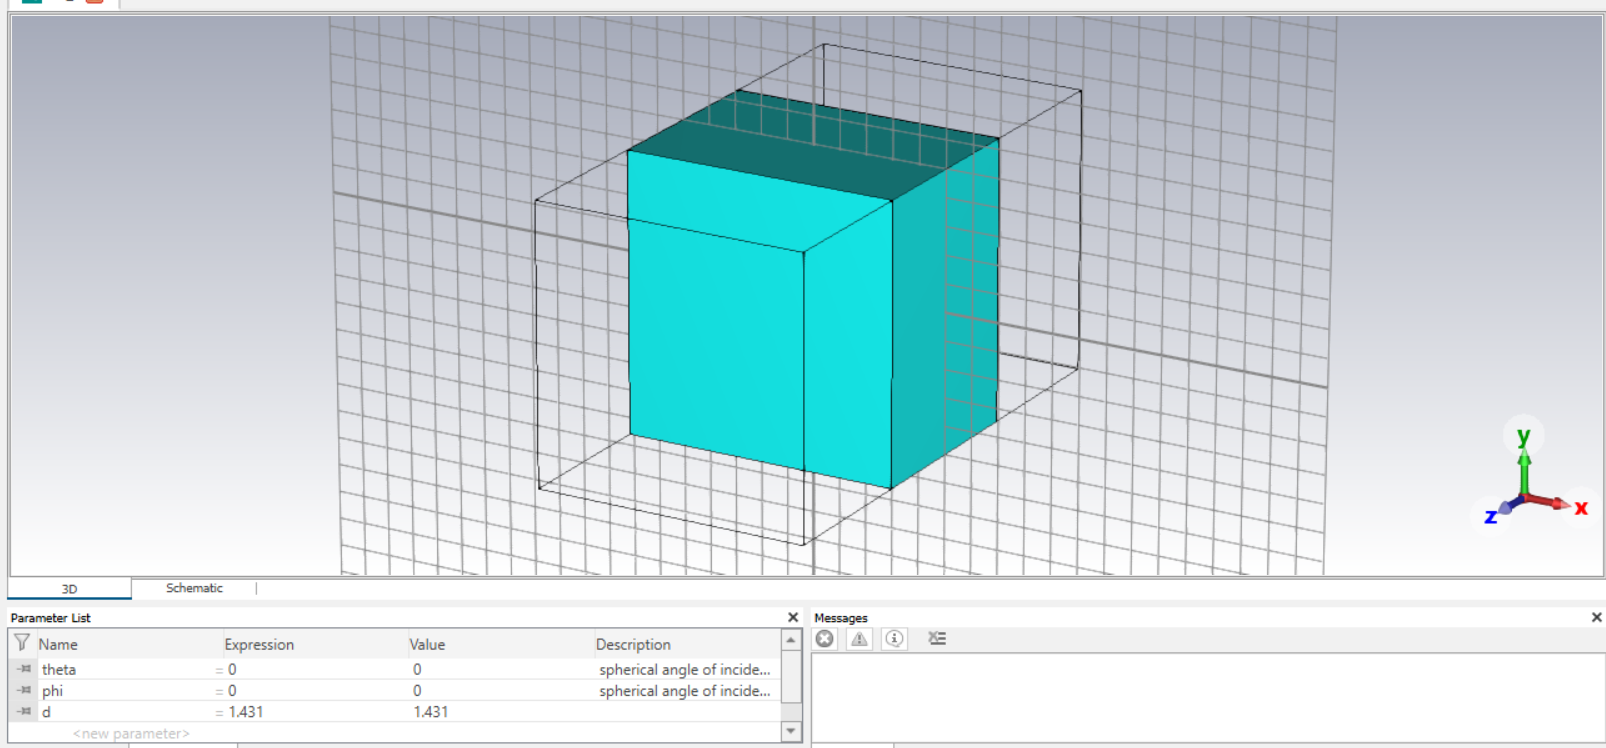
\includegraphics[width=0.75\textwidth]{img/structure.png}
		\caption{نمای ساختار مکعب دی‌الکتریک رسم شده در نرم‌افزار \lr{CST}}
		\label{fig:structure}
	\end{figure}
	
	\subsection{کد تحلیلی متلب و استخراج داده‌ها}
	پس از اجرای شبیه‌سازی در پهنای باند ۳۰ درصدی حول فرکانس مرکزی (۶۵ گیگاهرتز)، خروجی‌های مربوط به پارامترهای پراکندگی (ضریب بازتاب و عبور) به صورت فایل‌های متنی (\lr{.txt}) از نرم‌افزار \lr{CST} استخراج گردید. جهت محاسبه‌ی روابط تئوری استخراج‌شده در بخش قبل -- یعنی معادلات (۴) تا (۷) -- برای حالت با تلفات و در کل بازه‌ی فرکانسی شبیه‌سازی، و همچنین مقایسه‌ی آن با خروجی‌های عددی حاصل از حل کامل معادلات ماکسول در \lr{CST}، کد متلب زیر توسعه داده شده است. این کد داده‌های متنی استخراج‌شده را فراخوانی کرده، ضرایب بازتاب و عبور تحلیلی را به‌ازای هر فرکانس محاسبه می‌کند و نمودارهای تحلیلی و شبیه‌سازی را در کنار یکدیگر رسم می‌کند:
	
	\lr{\lstinputlisting[language=MATLAB, caption={\lr{Question 1}}, showstringspaces=false, basicstyle=\ttfamily, backgroundcolor=\color{yellow!15!white}, breaklines=true]{./code/FW_HW1_Q1.m}}
	
	\subsection{نتایج شبیه‌سازی و مقایسه نمودارها}
	با اجرای کد متلب فوق روی داده‌های استخراج شده، نمودارهای ضریب بازتاب ($S_{11}$) و ضریب عبور ($S_{21}$) رسم شدند. شکل‌های \ref{fig:s11} و \ref{fig:s21} تطابق دقیق مقادیر تئوری محاسبه شده در متلب را با نتایج شبیه‌سازی در \lr{CST} نشان می‌دهند؛ این تطابق، صحت مدل تحلیلی مبتنی بر خط انتقال معادل و همچنین صحت تنظیمات شبیه‌سازی (به‌ویژه پیکربندی پورت‌های فلوکه و شرایط مرزی متناوب) را تأیید می‌کند. همان‌طور که انتظار می‌رود، $S_{11}$ در فرکانس مرکزی طراحی به کمینه‌ی مقدار خود (نزدیک به صفر) و $S_{21}$ به بیشینه‌ی مقدار خود (نزدیک به یک، یا معادلاً نزدیک به $0$ دسی‌بل) می‌رسد. با دور شدن فرکانس از $f_c$ در هر دو سمت باند، شرط طول الکتریکی نیم‌موج ($\beta_2 d = \pi$) دیگر برقرار نیست، مکانیزم بازتولید امپدانس بار مختل می‌شود و در نتیجه دامنه‌ی $S_{11}$ به‌طور تدریجی افزایش و دامنه‌ی $S_{21}$ کاهش می‌یابد؛ رفتاری که پاسخ فرکانسی مشخصه‌ی این‌گونه مبدل‌های تک‌لایه (باند نسبتاً محدود اطراف فرکانس طراحی) را به نمایش می‌گذارد.
	
	\begin{figure}[H]
		\centering
		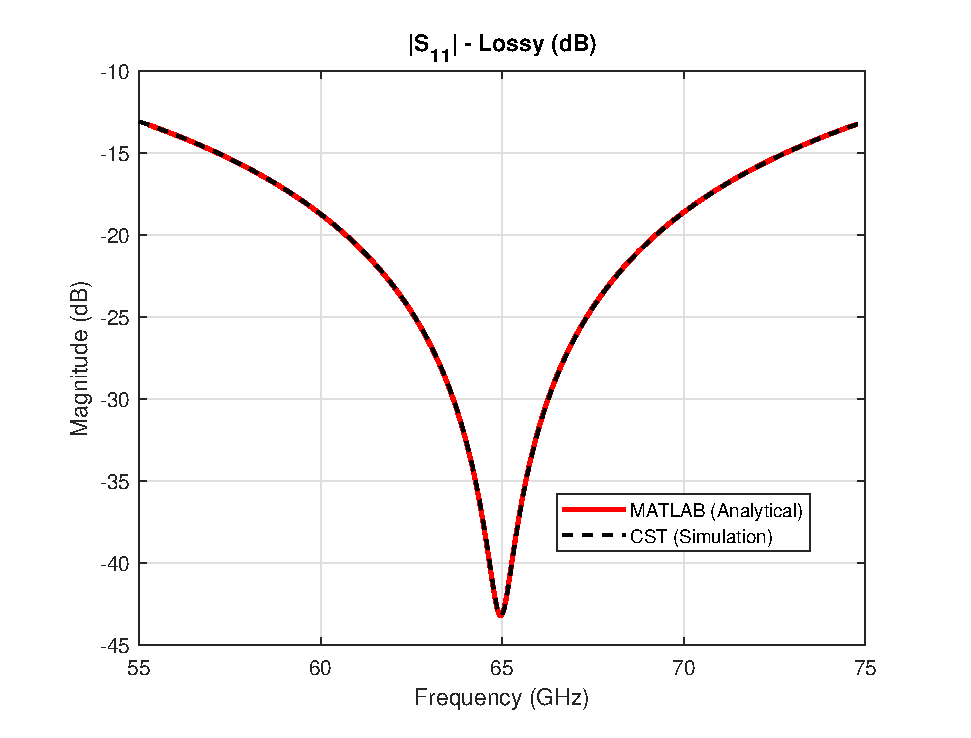
\includegraphics[width=0.7\textwidth]{img/S11_plot.eps}
		\caption{مقایسه ضریب بازتاب ($S_{11}$) تحلیلی متلب و شبیه‌سازی \lr{CST}}
		\label{fig:s11}
	\end{figure}
	
	\begin{figure}[H]
		\centering
		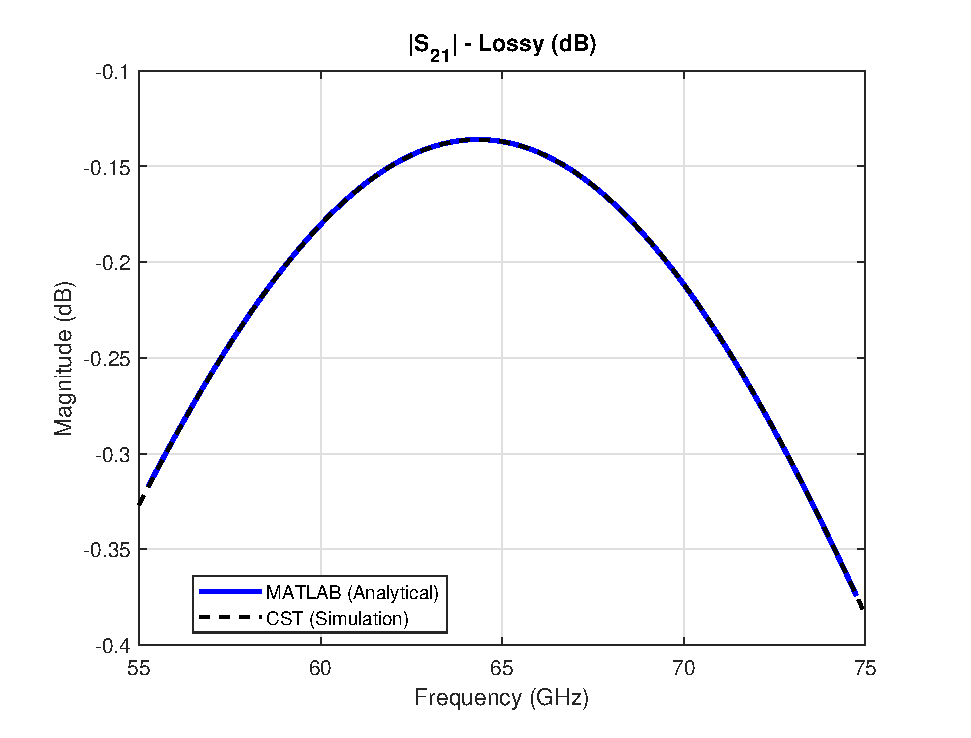
\includegraphics[width=0.7\textwidth]{img/S21_plot.eps}
		\caption{مقایسه ضریب عبور ($S_{21}$) تحلیلی متلب و شبیه‌سازی \lr{CST}}
		\label{fig:s21}
	\end{figure}
	
	\subsection{توزیع میدان‌های الکتریکی و انتشار امواج}
	جهت بررسی بصری نحوه انتشار امواج و عملکرد مبدل نیم موج، توزیع میدان الکتریکی (\lr{E-Field}) در مقطع عرضی ساختار برای سه فرکانس ابتدا، میانی و انتهای باند (پنجره ۳۰ درصدی حول ۶۵ گیگاهرتز) بررسی شده است. با توجه به پهنای باند، فرکانس ابتدایی حدود $55 \text{ GHz}$، فرکانس میانی $65 \text{ GHz}$ و فرکانس انتهایی $75 \text{ GHz}$ در نظر گرفته شده‌اند.
	
	در فرکانس میانی ($65 \text{ GHz}$)، همان‌طور که در بخش تئوری استدلال شد، ضخامت دی‌الکتریک دقیقاً معادل نیم طول موج راهنما است و بازتاب معادل ساختار به کمینه‌ی خود می‌رسد. از این رو انتظار می‌رود توزیع میدان در محیط اول (سمت فرودی) عمدتاً یک موج پیش‌رونده‌ی خالص با دامنه‌ی تقریباً ثابت باشد -- نشانه‌ی نبود موج ایستاده‌ی محسوس ناشی از بازتاب -- در حالی که در محیط سوم (سمت عبوری)، دامنه‌ی میدان تقریباً با دامنه‌ی موج فرودی برابر است که مؤید عبور تقریباً کامل انرژی از ساختار است. در فرکانس‌های ابتدایی و انتهایی باند، از آنجا که شرط نیم‌موج به‌طور دقیق برقرار نیست، الگوی تداخل موج فرودی و موج بازتابیده در محیط اول به‌صورت یک موج ایستاده‌ی جزئی (\lr{Partial Standing Wave}) با نسبت موج ایستاده‌ی بزرگ‌تر از یک نمایان می‌شود که در تصاویر میدان قابل مشاهده است.
	
	\begin{figure}[H]
		\centering
		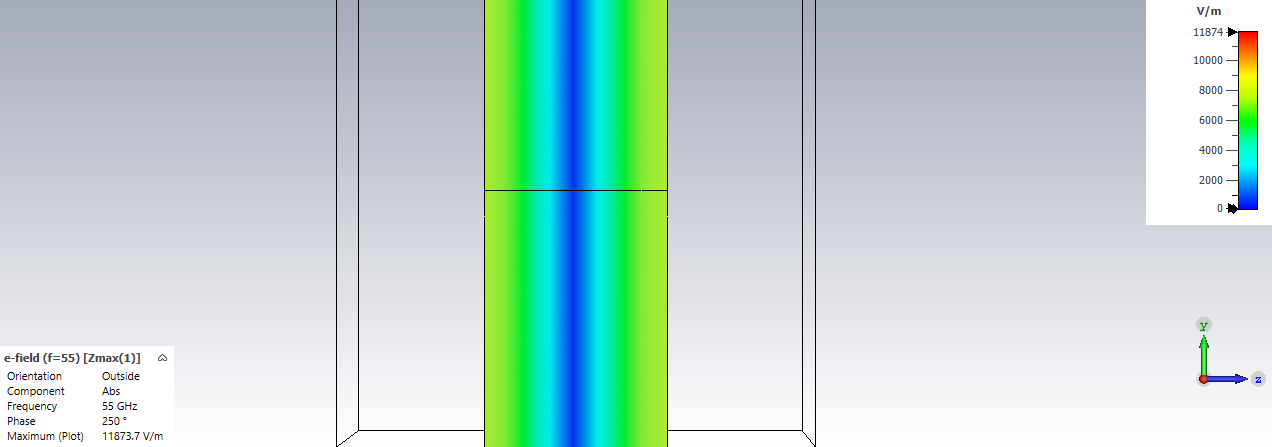
\includegraphics[width=0.7\textwidth]{img/55GHz}
		\caption{توزیع میدان الکتریکی و انتشار موج در فرکانس ابتدایی باند ($f = 55 \text{ GHz}$)}
		\label{fig:efield_start}
	\end{figure}
	
	\begin{figure}[H]
		\centering
		\includegraphics[width=0.7\textwidth]{img/65GHz} 
		\caption{توزیع میدان الکتریکی و انتشار موج در فرکانس میانی و تشدید ساختار ($f = 65 \text{ GHz}$)}
		\label{fig:efield_mid}
	\end{figure}
	
	\begin{figure}[H]
		\centering
		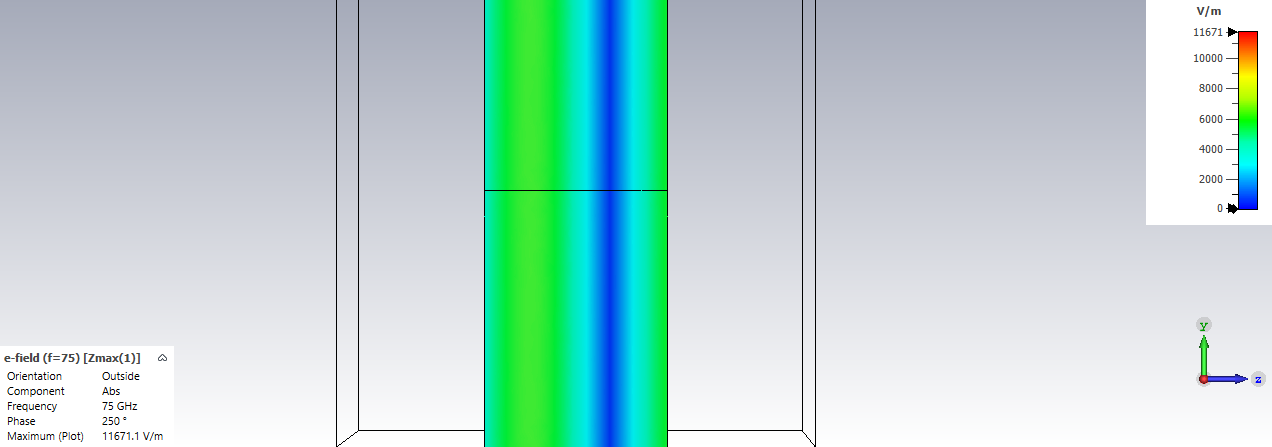
\includegraphics[width=0.7\textwidth]{img/75GHz}
		\caption{توزیع میدان الکتریکی و انتشار موج در فرکانس انتهایی باند ($f = 75 \text{ GHz}$)}
		\label{fig:efield_end}
	\end{figure}
	
	
	\section{بخش دوم: شبیه‌سازی اثر عمق نفوذ در دی‌الکتریک}
	
	در این بخش، پدیده‌ی انتشار امواج الکترومغناطیسی در یک محیط دی‌الکتریک تلف‌دار شبیه‌سازی و ارزیابی می‌شود. برخلاف بخش اول که در آن هدف حذف کامل بازتاب و دستیابی به عبور بی‌تلفات بود، در اینجا محیط دوم را نیمه‌بی‌نهایت (\lr{Half-Space}) در نظر می‌گیریم تا مکانیزم تضعیف موج در عمق ماده به‌صورت مجزا و بدون تداخل بازتاب‌های مرز دوم بررسی شود. هنگام انتشار موج در محیط‌های دارای تلفات، میدان الکتریکی متناوب، دوقطبی‌های مولکولی ماده را وادار به نوسان می‌کند؛ به دلیل اصطکاک داخلی و لغزش فازی این دوقطبی‌ها نسبت به میدان اعمالی (که در قالب رسانایی مؤثر یا به‌طور معادل تانژانت تلفات مدل می‌شود)، بخشی از انرژی الکترومغناطیسی موج به‌طور پیوسته به گرما تبدیل شده و در نتیجه دامنه‌ی موج با پیشروی در عمق ماده به‌طور نمایی افت می‌کند. تانژانت تلفات ($\tan\delta$) معیاری کمّی برای بیان شدت این اتلاف نسبت به جابجایی خالص انرژی است. عمق نفوذ یا عمق پوسته ($\delta$) نیز به مسافتی گفته می‌شود که در آن دامنه‌ی میدان الکتریکی موج به میزان $e^{-1}$ (تقریباً ۳۷ درصد) مقدار اولیه‌ی خود در سطح مرز تقلیل می‌یابد؛ از آنجا که چگالی توان با مجذور دامنه‌ی میدان متناسب است، در همین مسافت، توان موج به میزان $e^{-2}$ (تقریباً ۱۳.۵ درصد) مقدار اولیه کاهش می‌یابد. این کمیت در کاربردهایی نظیر طراحی جاذب‌های امواج راداری، تعیین ضخامت مؤثر پوشش‌های حفاظت الکترومغناطیسی (\lr{EMI Shielding}) و مشخصه‌یابی مواد تلف‌دار در فرکانس‌های میلی‌متری اهمیت عملی دارد.
	
	\subsection{روابط تئوری}
	برای اعمال اثر تلفات در معادلات، گذردهی الکتریکی محیط به صورت یک عدد مختلط تعریف می‌شود:
	\begin{equation}
		\epsilon = \epsilon_0 \epsilon_r (1 - j\tan\delta)
	\end{equation}
	با استفاده از این رابطه، ثابت انتشار مختلط موج ($\gamma$) به دست می‌آید:
	\begin{equation}
		\gamma = \alpha + j\beta = j\omega\sqrt{\mu_0\epsilon}
	\end{equation}
	که در آن $\alpha$ ثابت تضعیف (بخش حقیقی $\gamma$) و $\beta$ ثابت فاز (بخش موهومی $\gamma$) است؛ به‌طوری‌که پروفیل فضایی-زمانی میدان الکتریکی موج تخت به‌صورت $E(z,t) = E_0\, e^{-\alpha z}\cos(\omega t - \beta z)$ نوشته می‌شود. جمله‌ی $e^{-\alpha z}$ مسئول افت نمایی دامنه با پیشروی در عمق $z$ است، در حالی که جمله‌ی نوسانی $\cos(\omega t - \beta z)$ صرفاً انتشار فاز موج را با سرعت فاز $v_p=\omega/\beta$ توصیف می‌کند. عمق نفوذ موج در محیط تلف‌دار مستقیماً از معکوس ثابت تضعیف استخراج می‌شود:
	\begin{equation}
		\delta = \frac{1}{\alpha}
	\end{equation}
	با توجه به رابطه‌ی (۹)، افزایش هر یک از پارامترهای $\epsilon_r$ یا $\tan\delta$ (و نیز افزایش فرکانس) به افزایش ثابت تضعیف $\alpha$ و در نتیجه کاهش عمق نفوذ $\delta$ می‌انجامد؛ بنابراین انتظار می‌رود محیط مورد بررسی در این بخش، با $\epsilon_r=9$ و $\tan\delta=0.17$ که به‌مراتب تلف‌دارتر از پلکسی‌گلاس بخش اول است، عمق نفوذی به‌مراتب کوچک‌تر از خود نشان دهد.
	
	\subsection{تنظیمات شبیه‌سازی در نرم‌افزار \lr{CST}}
	جهت بررسی عمق نفوذ، لازم است یک موج تخت \lr{TEM} خالص با تابش عمودی به مرز دی‌الکتریک تولید شود؛ چالش اصلی در این مسیر آن است که یک موجبر مستطیلی متعارف با دیواره‌های کاملاً هادی (\lr{PEC}) در تمامی چهار وجه جانبی، مد غالب خود (\lr{TE10}) را دارای فرکانس قطع (\lr{Cutoff Frequency}) و ساختار میدانی غیریکنواخت در مقطع عرضی می‌سازد که هیچ‌کدام با یک موج تخت آزاد یکسان نیست. برای غلبه بر این محدودیت، از روش دوم پیشنهاد شده -- ترکیب هوشمندانه‌ی دو نوع شرط مرزی متفاوت در دو جفت وجه جانبی -- استفاده گردید که مکانیزم فیزیکی آن در ادامه تشریح می‌شود.
	
	در این راستا، یک موج تخت با تابش عمودی به مرز یک دی‌الکتریک با گذردهی نسبی $\epsilon_r = 9$ و تانژانت تلفات $\tan\delta = 0.17$ تابانده شد. فرکانس مرکزی شبیه‌سازی $62 \text{ GHz}$ فرض شده و تحلیل در یک پهنای باند ۳۰ درصدی حول این فرکانس صورت گرفت.
	
	برای مهندسی و ایجاد شرایط انتشار موج \lr{TEM}، از مرزهای \lr{Electric} ($E_t=0$) در دو وجه مقابل هم (محور $X$) و مرزهای \lr{Magnetic} ($H_t=0$) در دو وجه دیگر (محور $Y$) استفاده شد. مرز الکتریکی، معادل یک دیواره‌ی هادی کامل (\lr{PEC})، مؤلفه‌های مماسی میدان الکتریکی را روی آن وجه صفر می‌کند؛ در حالی که مرز مغناطیسی، معادل یک دیواره‌ی هادی مغناطیسی کامل (\lr{PMC})، مؤلفه‌های مماسی میدان مغناطیسی را روی وجه مقابل صفر می‌سازد. اعمال هم‌زمان این دو نوع شرط مرزی متعامد، عملاً میدان الکتریکی را مجبور می‌کند تنها در راستای $x$ و میدان مغناطیسی را تنها در راستای $y$ نوسان کند و هرگونه وابستگی میدان‌ها به مختصات $x$ و $y$ را حذف می‌کند -- دقیقاً همان تقارنی که یک موج تخت یکنواخت با انتشار در راستای $z$ از خود بروز می‌دهد. از منظر تئوری خطوط انتقال، این پیکربندی معادل یک موجبر صفحات موازی (\lr{Parallel-Plate Waveguide}) باز است که برخلاف موجبر مستطیلی تمام-\lr{PEC}، فاقد فرکانس قطع بوده و مد \lr{TEM} را به‌عنوان مد غالب و بدون هیچ محدودیت فرکانسی پشتیبانی می‌کند؛ به همین دلیل، ساختار برای هر فرکانسی در باند شبیه‌سازی، صرفاً موج \lr{TEM} خالص را هدایت می‌کند و از آلودگی مدهای مرتبه‌ی بالاتر مبرا است.
	
	همچنین وجوه مربوط به محور انتشار ($Z_{min}$ و $Z_{max}$) به صورت \lr{Open} تنظیم شده و با استفاده از \lr{Waveguide Port} تحریک شدند تا انرژی موج بدون بازتاب مصنوعی از مرزهای محاسباتی وارد و خارج شود. اعمال همزمان شرایط مرزی الکتریکی و مغناطیسی در دیواره‌های جانبی، باعث می‌شود مؤلفه‌های طولی میدان‌ها ($E_z$ و $H_z$) به‌طور کامل حذف شده و یک موج \lr{TEM} خالص در راستای محور $Z$ منتشر شود که از نظر فیزیکی معادل دقیق یک موج تخت با تابش عمودی در فضای آزاد است و مقایسه‌ی مستقیم آن با روابط تحلیلی یک‌بعدی بخش قبل (معادلات ۸ تا ۱۰) را موجه می‌سازد.
	
	\begin{figure}[H]
		\centering
		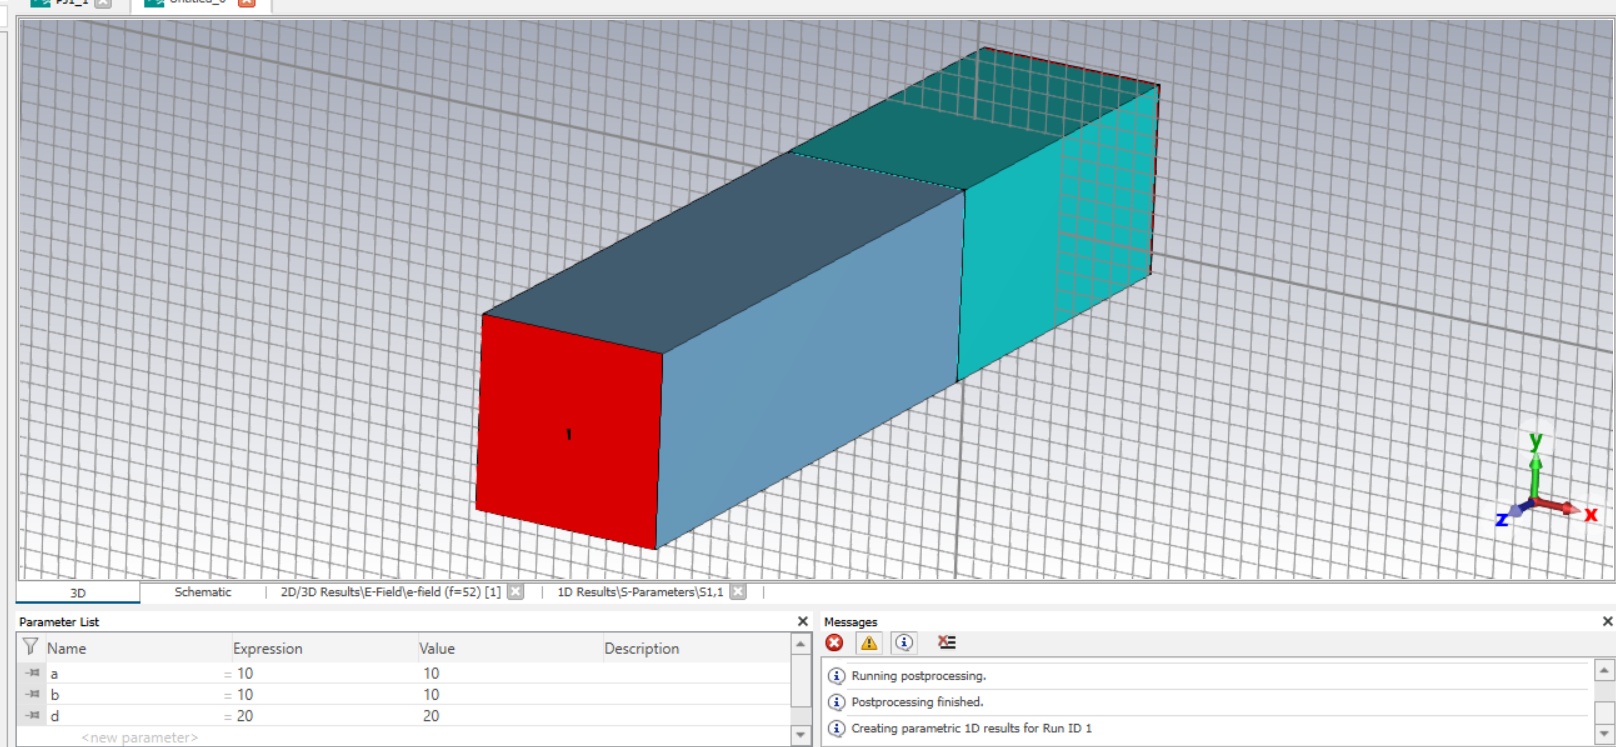
\includegraphics[width=0.75\textwidth]{img/Q2_structure.png}
		\caption{نمای سه‌بعدی ساختار شبیه‌سازی شده و تنظیمات مرزها در محیط \lr{CST}}
		\label{fig:q2_structure}
	\end{figure}
	\subsection{استخراج عمق نفوذ در محیط \lr{Post-Processing}}
	برای اندازه‌گیری مستقیم عمق نفوذ از روی میدان‌های شبیه‌سازی شده، به‌جای اتکا بر برازش یک منحنی نمایی کامل بر پروفیل میدان، از یک روش نقطه‌ای و مستقیم استفاده شد: دو پروب میدان (\lr{Field Probe}) در راستای انتشار موج قرار داده شد. پروب اول دقیقاً روی مرز دی‌الکتریک ($Z_1$) و پروب دوم با فاصله مشخص یک میلی‌متر در داخل محیط تلف‌دار ($Z_2$) تعبیه گردید. از آنجا که در یک محیط همگن، دامنه‌ی میدان دقیقاً به‌صورت تابع نمایی $|E(z)|=|E_0|e^{-\alpha z}$ افت می‌کند، نسبت دامنه‌ی میدان در دو نقطه‌ی شناخته‌شده به‌طور مستقیم ثابت تضعیف محلی $\alpha$ و از آن، عمق نفوذ را نتیجه می‌دهد. با استفاده از ابزار \lr{Mix Template Results} در نرم‌افزار، عمق نفوذ در کل بازه فرکانسی از طریق رابطه زیر ارزیابی شد:
	\begin{equation}
		\delta = \frac{\Delta z}{\ln(|E_1|/|E_2|)}
	\end{equation}
	که در آن $\Delta z = 1 \text{ mm}$ فاصله بین دو پروب می‌باشد.
	
	\subsection{کد تحلیلی متلب و بررسی نتایج}
	به منظور محاسبه دقیق مقادیر تئوری $\alpha$ و $\delta$ (بر اساس معادلات ۸ تا ۱۰) و همچنین پارامترهای پراکندگی ($S_{11}$ و $S_{21}$) ناشی از بازتاب جزئی در مرز هوا-دی‌الکتریک، کد متلب زیر توسعه یافته است. در این کد محاسبات درون یک حلقه \lr{for} به ازای تمامی فرکانس‌های باند انجام شده -- با این فرض که تانژانت تلفات ماده در بازه فرکانسی شبیه‌سازی تقریباً ثابت می‌ماند -- و سپس با داده‌های خروجی نرم‌افزار \lr{CST} مقایسه می‌گردند:
	
	\lr{\lstinputlisting[language=MATLAB, caption={\lr{Question 1}}, showstringspaces=false, basicstyle=\ttfamily, backgroundcolor=\color{yellow!15!white}, breaklines=true]{./code/FW_HW1_Q2.m}}
	
	\subsection{نمودارهای مقایسه تئوری و شبیه‌سازی}
	شکل‌های زیر مقایسه تطبیقی بین خروجی‌های تحلیلی کد متلب و داده‌های استخراج شده از شبیه‌سازی \lr{CST} را در کل پهنای باند نمایش می‌دهند. تطابق نمودارهای $S_{11}$ و $S_{21}$ (شکل‌های \ref{fig:q2_s11} و \ref{fig:q2_s21}) صحت مدل تک‌بعدی مبتنی بر امپدانس ذاتی مختلط را برای پیش‌بینی بازتاب جزئی موج از سطح یک محیط نیمه‌بی‌نهایت تلف‌دار تأیید می‌کند. در نمودار عمق نفوذ (شکل \ref{fig:q2_skindepth}) نیز روند کاهشی $\delta$ با افزایش فرکانس در طول باند قابل مشاهده است؛ این روند مستقیماً از رابطه (۹) نتیجه می‌شود، چرا که ثابت تضعیف $\alpha$ (و در نتیجه معکوس آن، $\delta$) به‌طور خطی با فرکانس زاویه‌ای $\omega$ مقیاس می‌شود و از این رو در فرکانس‌های میلی‌متری بالاتر، موج در فاصله‌ای کوتاه‌تر از سطح مرز به‌طور مؤثر میرا می‌شود.
	
	\begin{figure}[H]
		\centering
		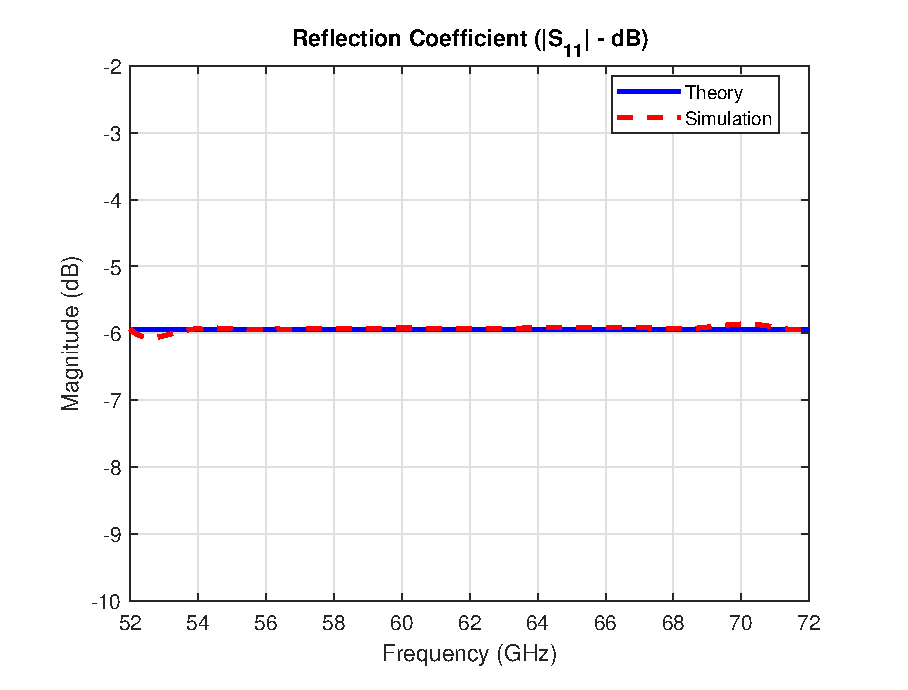
\includegraphics[width=0.7\textwidth]{img/Q2_S11_plot.eps}
		\caption{مقایسه ضریب بازتاب ($S_{11}$) تئوری و شبیه‌سازی برای دی‌الکتریک تلف‌دار}
		\label{fig:q2_s11}
	\end{figure}
	
	\begin{figure}[H]
		\centering
		\includegraphics[width=0.7\textwidth]{img/Q2_S21_plot.eps}
		\caption{مقایسه ضریب عبور ($S_{21}$) تئوری و شبیه‌سازی}
		\label{fig:q2_s21}
	\end{figure}
	
	\begin{figure}[H]
		\centering
		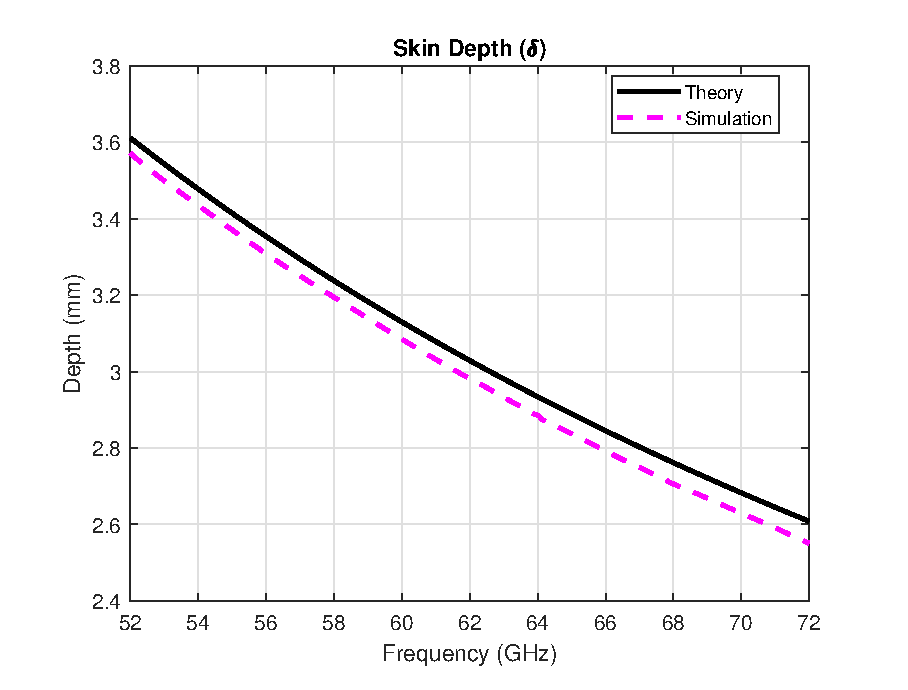
\includegraphics[width=0.7\textwidth]{img/Q2_SkinDepth_plot.eps}
		\caption{مقایسه تغییرات عمق نفوذ ($\delta$) بر حسب فرکانس}
		\label{fig:q2_skindepth}
	\end{figure}
	
	\subsection{توزیع میدان الکتریکی}
	برای مشاهده عینی پدیده تضعیف و محاسبه عمق نفوذ، توزیع میدان الکتریکی در سطح مقطع عرضی ساختار در سه فرکانس ابتدا، میانی و انتهای باند (پنجره ۳۰ درصدی حول ۶۲ گیگاهرتز) بررسی شده است. فرکانس ابتدایی معادل $52 \text{ GHz}$، فرکانس مرکزی $62 \text{ GHz}$ و فرکانس انتهایی $72 \text{ GHz}$ در نظر گرفته شده‌اند. همان‌طور که در تصاویر مشخص است، دامنه موج بلافاصله پس از عبور از مرز و ورود به دی‌الکتریک، با پیشروی در عمق ماده به شدت افت کرده و ظرف فاصله‌ای معادل چند برابر $\delta$ عملاً محو می‌شود؛ این محلی‌سازی انرژی الکترومغناطیسی در لایه‌ای نازک نزدیک سطح، همان اصلی است که مبنای کاربردهای عملی این پدیده در طراحی جاذب‌های راداری و پوشش‌های حفاظتی الکترومغناطیسی قرار می‌گیرد. با مقایسه کیفی سه تصویر، کاهش تدریجی طول مؤثر نفوذ موج با افزایش فرکانس از $52$ به $72 \text{ GHz}$ نیز به‌وضوح قابل تشخیص است که با روند پیش‌بینی‌شده در شکل \ref{fig:q2_skindepth} هم‌خوانی دارد.
	
	\begin{figure}[H]
		\centering
		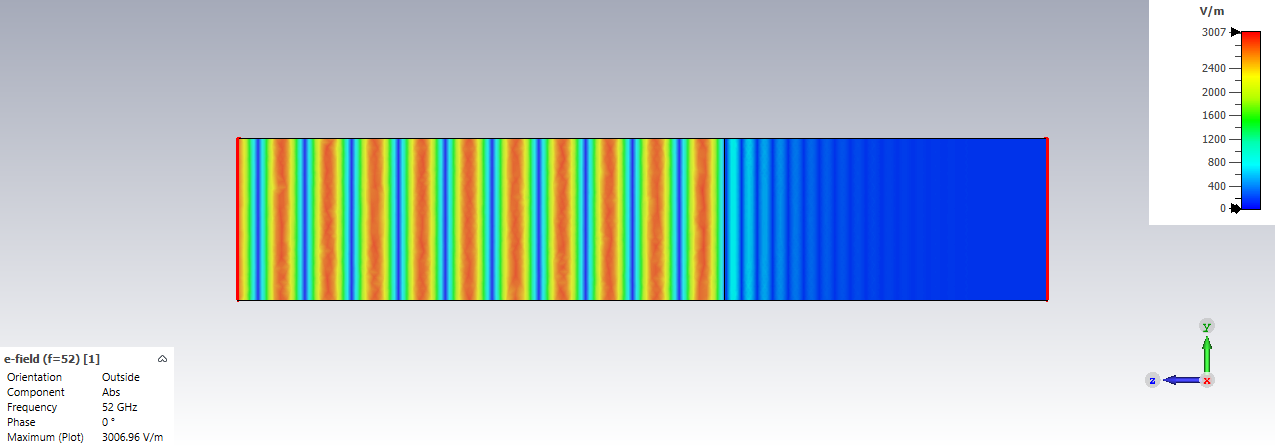
\includegraphics[width=0.7\textwidth]{img/Q2_Efield_Start}
		\caption{توزیع میدان الکتریکی و تضعیف موج در فرکانس ابتدایی باند ($f = 52 \text{ GHz}$)}
		\label{fig:q2_efield_start}
	\end{figure}
	
	\begin{figure}[H]
		\centering
		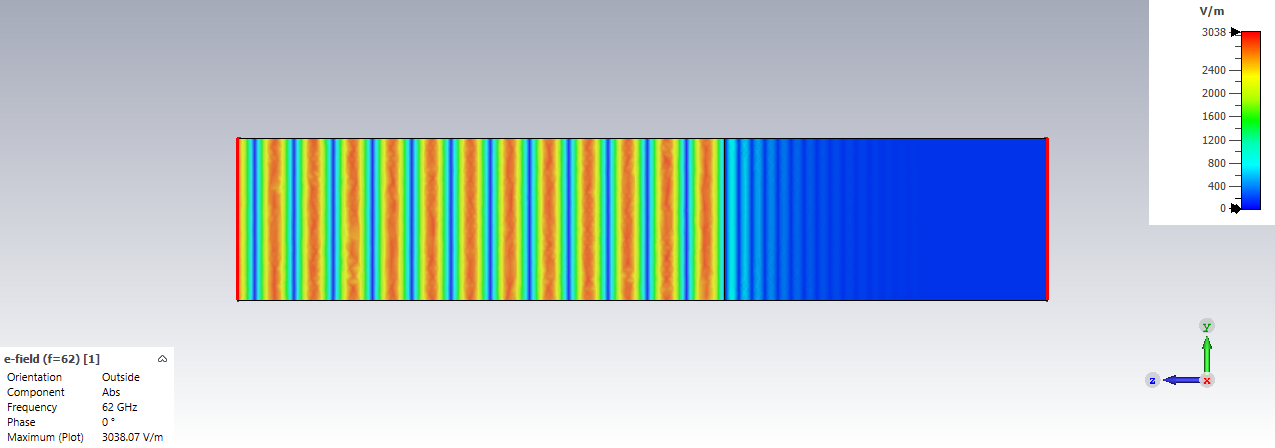
\includegraphics[width=0.7\textwidth]{img/Q2_Efield_Mid} 
		\caption{توزیع میدان الکتریکی و تضعیف موج در فرکانس مرکزی ($f = 62 \text{ GHz}$)}
		\label{fig:q2_efield_mid}
	\end{figure}
	
	\begin{figure}[H]
		\centering
		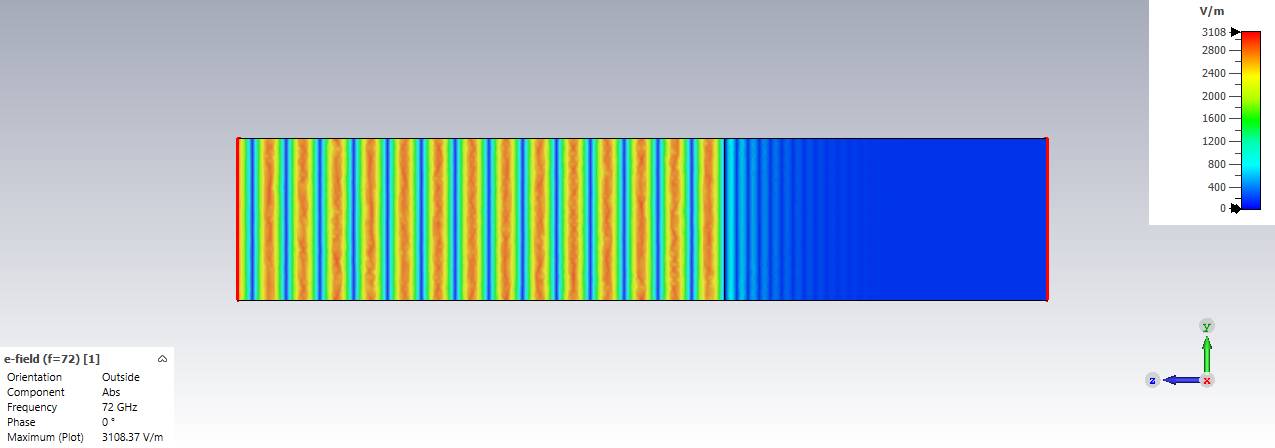
\includegraphics[width=0.7\textwidth]{img/Q2_Efield_End}
		\caption{توزیع میدان الکتریکی و تضعیف موج در فرکانس انتهایی باند ($f = 72 \text{ GHz}$)}
		\label{fig:q2_efield_end}
	\end{figure}
	
	\textbf{توجه:} فایل‌های متحرک (\lr{.gif}) مربوط به انتشار امواج در مقطع عرضی  به صورت مجزا آپلود گردیده‌اند.
	
	\clearpage
	\section{تحلیل فیزیکی و مکانیزم ایجاد موج عرضی الکترومغناطیسی (\lr{TEM}) با شرایط مرزی ترکیبی}
	
	\textbf{سوال پروژه:} 
	اگر دو وجه مقابل هم را به صورت مرز الکتریکی ($E_t = 0$ یا \lr{minX/maxX}) و دو وجه دیگر را به صورت مرز مغناطیسی ($H_t = 0$ یا \lr{minY/maxY}) انتخاب کنیم و وجوه ورودی و خروجی (\lr{minZ/maxZ}) را روی حالت \lr{Open} قرار دهیم، ساختار با موج \lr{TEM} تحریک می‌شود. دلیل فیزیکی این پدیده چیست؟
	
	\paragraph{پاسخ تحلیلی و فیزیکی:}
	برای درک علت این پدیده، باید ویژگی‌های بنیادی یک موج عرضی الکترومغناطیسی (\lr{TEM}) و نحوه تاثیر شرایط مرزی بر مولفه‌های میدان را بر اساس معادلات ماکسول بررسی کنیم. یک موج \lr{TEM} خالص که در راستای محور $Z$ منتشر می‌شود، موجی است که هیچ مؤلفه میدانی در راستای انتشار ندارد؛ یعنی هم میدان الکتریکی و هم میدان مغناطیسی کاملاً بر راستای انتشار عمود هستند:
	\begin{equation}
		E_z = 0 , \quad H_z = 0
		\end{equation}
	در چنین موجی، اگر میدان الکتریکی را در راستای محور $X$ ($E = E_x \hat{x}$) فرض کنیم، بر اساس رابطه پوینتینگ و عمود بودن میدان‌ها، میدان مغناطیسی ناگزیر در راستای محور $Y$ ($H = H_y \hat{y}$) قرار خواهد گرفت.
	
	اعمال شرایط مرزی ترکیبی (\lr{PEC/PMC}) در دیواره‌های جانبی، این الگوی میدان را به دلایل زیر در داخل یک فضای محدود زنده و پایدار نگه می‌دارد:
	
	\begin{enumerate}
		\item \textbf{نقش مرزهای الکتریکی کامل (\lr{PEC} یا $E_t=0$):} 
		هنگامی که وجوه \lr{minX} و \lr{maxX} را به عنوان مرز الکتریکی تعریف می‌کنید، شرط مرزی حکم می‌کند که مؤلفه‌های مماس بر این صفحات (یعنی $E_y$ و $E_z$) باید دقیقاً صفر شوند. این شرط به میدان الکتریکی اجازه می‌دهد که به صورت کاملاً عمود بر این دیواره‌ها (یعنی در راستای $\hat{x}$) وجود داشته باشد. از طرفی، این دیواره‌ها برای میدان مغناطیسی مماس ($H_y$) مانند یک هادی ایده‌آل عمل کرده و خطوط میدان مغناطیسی به راحتی به صورت مماس بر آن جریان می‌یابند بدون آنکه مخدوش شوند.
		
		\item \textbf{نقش مرزهای مغناطیسی کامل (\lr{PMC} یا $H_t=0$):}
		هنگامی که وجوه \lr{minY} و \lr{maxY} را به عنوان مرز مغناطیسی تعریف می‌کنید، شرط مرزی مماس بودن میدان مغناطیسی را سرکوب می‌کند؛ یعنی مؤلفه‌های $H_x$ و $H_z$ روی این وجوه باید صفر شوند. این امر باعث می‌شود میدان مغناطیسی مجبور شود تنها به صورت عمود بر این صفحات (در راستای $\hat{y}$) آرایش یابد. در عین حال، میدان الکتریکی مماس ($E_x$) بدون هیچ محدودیتی می‌تواند به صورت مماس بر این دیواره‌های مغناطیسی قرار گیرد.
		

	\end{enumerate}
	
	
	\vfill
	\begin{flushleft}
		\Huge\textbf{مرسی از توجه شما}
	\end{flushleft}
\end{document}